% !TEX root = ../thesis.tex
\chapter{Overview}
\label{chapter:<Overview>}
\ldots

\acresetall

This   chapter   will   simply   expose   to   the   reader   some   background 
necessary adopted on this research. Basic concepts of recommendation systems, its 
algorithms, explanations and layouts might be of knowledge of the one in hand 
of this project description, but a brief review could be useful to understand the 
whole application design.

\section{Introduction}

Before going through all the known algorithms it is worth for the reader know some basic notions about a recommendation system.

With the emerging of hardware resources and computational power recommendation system have grown and diversified. Just decades ago a recommendation would have taken hundreds of mainframes to be completed. Nowadays with hardware as a commodity and all the emerging cloud solutions that allows to have the amount of desired computational power, RAM and storage for just the time requested, deploying recommendation system has never been faster and cheaper. Also big companies like Netflix completely run on cloud systems like the one by Amazon or Rackspace. 
As soon as internet and computers evolved and more information was available and interconnected, search engine started to arise and being adopted by the newborn internet community. These early search engines were basically of two types \cite{spiegazione_confidenza_raccomandazione}:
\begin{itemize}
\item Information retrieval. A keyword is the base concept of this type. Keyword or a set of keywords are used to look for the desired content. The points of failure of this kind of search may be the chosen keyword. In fact the content could have been categorized used a set of different keywords that the one the user is looking for, thus the content is not selected even if it is relevant to the user.
\item Information filtering. Preferences established by the user are used as a background knowledge to select the relevant items for the user or, alternatively, properties of a item or a subset of items can be used to lead to another set of relevant items.
\end{itemize}

Recommendation systems are basically of the second type or information retrieval and they evolved heavily under all 90'. Nowadays search engine giants like Google or Yahoo use both types in integrated system to lead to stronger and valuable results. Lately with the adoption of smart phones and tablets which have a small screen size and different human-computer interaction than a traditional personal computer with a mouse and a keyboard, recommendation systems to surf content on those devices are critical applications and under heavily development. 

Recommendation system are widely adopted in all the most known website and web applications. They may be based on 
\begin{itemize}
\item User profile: the recommendation is based on information gathered from the user. The information can be explicit or implicit. An example of explicit information is the set of ratings. Supposing we are in the case of a movie web application the user profile is the list of all the ratings that the user made for each movie in the database. An example of implicit is the set of pages or items that the user viewed, in the case of a movie web application this can be just the list of items that the user viewed during the continuous navigation of the website.
\item Item content: the recommendation is based on the current item or set of item displayed. In this case no information about the user is used by the algorithm. As and example of this scenario for a web application abut movies, the item content for the recommendation can be the name of the actors, the genre, the release date or the plot description.
\end{itemize}

We should see a recommendation system as a complementary system of a search engine and not a different implementation of a concept of a search engine. They solve two different problems. Search engines are really powerful when the user knows or has an idea of what he or she is looking for. The user types a keyword or a set of keyword in a text field and the algorithms involved select the contents relevant for that search.
Recommendation system are useful when the user actually does not know what she or he is looking for. Their added value is in suggesting an item that may be interesting from the user perspective. The user has not a keyword to start his/her navigation with. he/she will just receive the new item, maybe without even asking about it. Since search engines and recommendation systems solve different problems they are often implemented one aside the other to keep the user in the web application or to satisfy user's needs. From a research \cite{usercentric_evaluation_framework} at RecSys \cite{recsys}, 45\% of users will likely shop in a web application that employs recommendation technology and 69\% of users in the highest spending category are more likely to desire the support of recommendation technology during their web application navigation or shopping. So recommendation systems are valuable from both user and web application. It offers the benefit of an easy way to navigate and find items for an user and a better service and/or a better shopping experience for the web application.

\section{Analysis}
\label{sec:Analysis}

Recommendation systems, like search engines, are very complex systems with a strong time constraints. From a recent study \cite{page-abandonment} users often leave web pages in 10-20 seconds but pages with a clear value proposition can hold people's attention for much longer because visit-durations follow a negative Weibull distribution. Due to this nature of the web user pages should load as quick as possible and thus search results or recommendation results should be displayed in no more than few seconds or the user will leave the page without even looking at the results. These kind of constraints have influenced the way recommendation systems have been developed and evolved through time.
From a black box point of view a recommendation system is just a tool that given the proper input returns an output. No matter which algorithm, programming language, or added feature the recommendation system applies, all recommendation system analyzed respect this constraint. Given that we will explore the input of a recommendation system and its stack. The algorithms can be categorized in two families depending from the requested input:

\begin{itemize}
\item Content based.
\item Collaborative.
\end{itemize}

\subsection{Input}
\label{sec:Input}

There are two kind of inputs for a recommendation system \cite{thesis-andreia}. 
\begin{itemize}
\item Item content matrix. It is used in content based algorithms. It is a matrix which has all the items as columns and all the metadata as rows. A metadata is a specific characteristic or feature which may be present or may not be present for the given item. In case of the metadata being present in the given item the corresponding cell is set to 1, 0 otherwise. In a case of a recommendation system for movies the metadata could be the presence of an actor, the set of genres and keywords extracted from the plot. Figure \ref{fig:ICM} shows how items and metadata correlate in the composition of the item content matrix.

  \begin{figure}
    \centering
    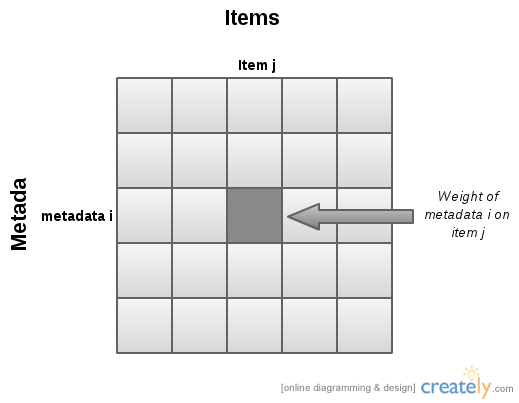
\includegraphics[width=0.7\textwidth]{figures/ICM.png}
    \caption{ICM}
    \label{fig:ICM}
  \end{figure}
 
\item User rating matrix. It's used for collaborative algorithms. It is a matrix which has all the items as columns and all the users as rows. The cell identified by a item and a user contains the rating that the user gave to that movie. It has the value of 0 if there is not any rating for the given item. To better clarify the composition of an user rating matrix, the figure \ref{fig:URM} explains how it is composed.

  \begin{figure}
    \centering
    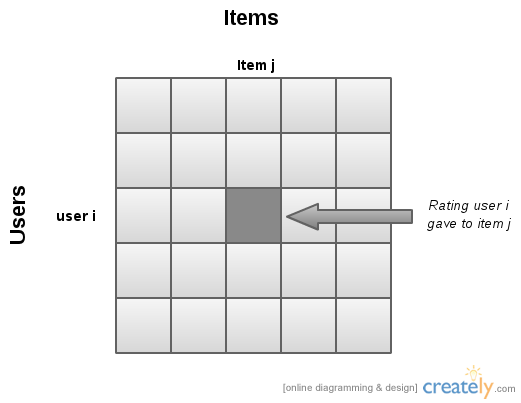
\includegraphics[width=0.7\textwidth]{figures/URM.png}
    \caption{URM}
    \label{fig:URM}
  \end{figure}

The rating can be collected in two different ways:
\begin{itemize}
\item Explicitly. The user is aware that he/she is rating an item. The rating can be provided in different scales. The most common scales are: binary, 3-scale or 5-scale. Binary is a two value rating usually referred as `like` or `dislike`. 3-scale is usually referred as 3 stars or 3 thumbs up. 5-scale is usually referred as 5 stars or a slicer in the 0-5 range. In all the scales, low rating means that the user disliked the item, high values mean that the user liked the item.
\item Implicit. The user is not aware that he/she is rating an item. While browsing the system collect navigation information like clicks on links or displayed pages and based on this information implies ratings for the items. This way of collecting data is very used nowadays with pervasive web applications. Information is key point in business. The more a company know about its customers the better it will be able in satisfy their expectations. 
\end{itemize}
\end{itemize}

\subsection{Stack}
\label{sec:Stack}

 To make this possible recommendation system evolved in a stack like way that can be summarized in three phases:
\begin{itemize}
\item Batch or model creation
\item Real time or recommendation generation
\item Antireshuffling or recommendation update 
\end{itemize}
